% a-ab.tex

% !TEX program = pdflatex
\documentclass[tikz]{standalone}
\usepackage{amsmath}
\usepackage{tikz}
\usetikzlibrary{arrows,automata}

\begin{document}
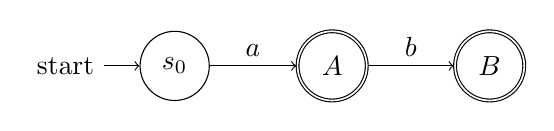
\begin{tikzpicture}[->, auto, node distance = 2cm]
  \node[state, initial] (init) {$s_{0}$};
  \node[state, accepting] (A) [right of = init] {$A$};
  \node[state, accepting] (B) [right of = A] {$B$};

  \path (init) edge node {$a$} (A)
        (A) edge node {$b$} (B);
\end{tikzpicture}
\end{document}